\documentclass[../main]{subfiles}
\begin{document}

\graphicspath{{../figures/}}

\section{検証実験}
本研究では,提案手法の有効性を検証するために,全方向マイクを搭載した台車を移動ロボットに見立て,横約2.3m,縦約3.3mの経路を走行させ,異常音源の座標を推定する実験を行った.
正常音のデータは,全てのギアボックスから正常な運転音を収録したものを用い,異常音のデータは,正常音の収録の際に使用したギアボックスのうち一つにのみ,
歯車に異物を接触させることで発生した音を収録したものを用いた.
経路には,10個のギアボックスを,それぞれ経路から30cm離れた場所に音源として配置した.
\reffig{route}に移動ロボットの経路とギアボックスの音源の配置を示す.
また異常音源は,\reffig{route}に示す経路の(0.50m,-0.30m)に配置した.


正常音のデータと異常音のデータの取得回数はそれぞれ4セットと1セットであり,それぞれ105秒間収録した.尚,正常音のデータのうち3セットを学習データ,1セットを検証データとして用いた.


実験に用いたマイクのサンプリング周波数は48.0kHz,前処理に用いた短時間フーリエ変換のウィンドウサイズは65536,スライド幅は1024,メルフィルタバンクの数は128とした.
また取得したデータの低周波成分に,ロボットの移動が由来と思われる非定常なノイズが含まれたことから,予測モデルの学習時には,データの前処理として,1khz以上の周波成分のみに対応する特徴量を使用した.

また,正常音のマッピングに用いたニューラルネットワークの構造は,中間層5層に対し,各層のノード数はそれぞれ4, 8, 16, 32, 64とし,これらの層を全結合層で構成した.

\begin{figure}[tb]
  \centering
  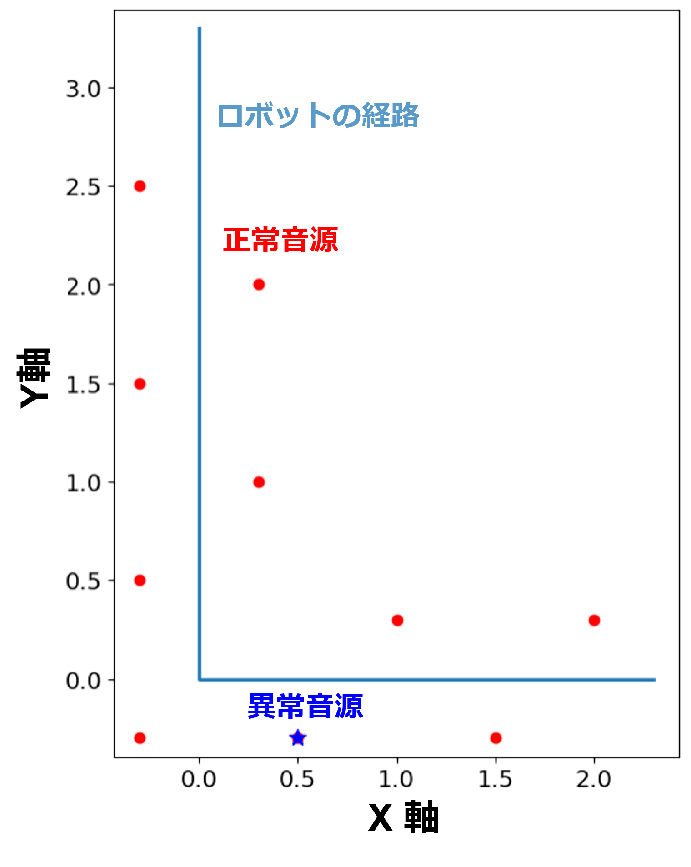
\includegraphics[keepaspectratio, width=0.8\linewidth]{route.pdf}
  \caption{移動ロボットの経路と音源の配置}
  \labfig{route}
\end{figure}

\end{document}
